\documentclass[
  bibliography=totoc,     % Literatur im Inhaltsverzeichnis
  captions=tableheading,  % Tabellenüberschriften
  titlepage=firstiscover, % Titelseite ist Deckblatt
]{scrartcl}

% Paket float verbessern
\usepackage{scrhack}

% Warnung, falls nochmal kompiliert werden muss
\usepackage[aux]{rerunfilecheck}

% unverzichtbare Mathe-Befehle
\usepackage{amsmath}
% viele Mathe-Symbole
\usepackage{amssymb}
% Erweiterungen für amsmath
\usepackage{mathtools}

% Fonteinstellungen
\usepackage{fontspec}
% Latin Modern Fonts werden automatisch geladen
% Alternativ zum Beispiel:
%\setromanfont{Libertinus Serif}
%\setsansfont{Libertinus Sans}
%\setmonofont{Libertinus Mono}

% Wenn man andere Schriftarten gesetzt hat,
% sollte man das Seiten-Layout neu berechnen lassen
\recalctypearea{}

% deutsche Spracheinstellungen
\usepackage{polyglossia}
\setmainlanguage{german}


\usepackage[
  math-style=ISO,    % ┐
  bold-style=ISO,    % │
  sans-style=italic, % │ ISO-Standard folgen
  nabla=upright,     % │
  partial=upright,   % ┘
  warnings-off={           % ┐
    mathtools-colon,       % │ unnötige Warnungen ausschalten
    mathtools-overbracket, % │
  },                       % ┘
]{unicode-math}

% traditionelle Fonts für Mathematik
\setmathfont{Latin Modern Math}
% Alternativ zum Beispiel:
%\setmathfont{Libertinus Math}

\setmathfont{XITS Math}[range={scr, bfscr}]
\setmathfont{XITS Math}[range={cal, bfcal}, StylisticSet=1]

% Zahlen und Einheiten
\usepackage[
  locale=DE,                   % deutsche Einstellungen
  separate-uncertainty=true,   % immer Fehler mit \pm
  per-mode=symbol-or-fraction, % / in inline math, fraction in display math
]{siunitx}

% chemische Formeln
\usepackage[
  version=4,
  math-greek=default, % ┐ mit unicode-math zusammenarbeiten
  text-greek=default, % ┘
]{mhchem}

% richtige Anführungszeichen
\usepackage[autostyle]{csquotes}

% schöne Brüche im Text
\usepackage{xfrac}

% Standardplatzierung für Floats einstellen
\usepackage{float}
\floatplacement{figure}{htbp}
\floatplacement{table}{htbp}

% Floats innerhalb einer Section halten
\usepackage[
  section, % Floats innerhalb der Section halten
  below,   % unterhalb der Section aber auf der selben Seite ist ok
]{placeins}

% Seite drehen für breite Tabellen: landscape Umgebung
\usepackage{pdflscape}

% Captions schöner machen.
\usepackage[
  labelfont=bf,        % Tabelle x: Abbildung y: ist jetzt fett
  font=small,          % Schrift etwas kleiner als Dokument
  width=0.9\textwidth, % maximale Breite einer Caption schmaler
]{caption}
% subfigure, subtable, subref
\usepackage{subcaption}

% Grafiken können eingebunden werden
\usepackage{graphicx}
% größere Variation von Dateinamen möglich
\usepackage{grffile}

% schöne Tabellen
\usepackage{booktabs}

% Verbesserungen am Schriftbild
\usepackage{microtype}

% Literaturverzeichnis
\usepackage[
  backend=biber,
]{biblatex}
% Quellendatenbank
\addbibresource{lit.bib}
\addbibresource{programme.bib}

% Hyperlinks im Dokument
\usepackage[
  unicode,        % Unicode in PDF-Attributen erlauben
  pdfusetitle,    % Titel, Autoren und Datum als PDF-Attribute
  pdfcreator={},  % ┐ PDF-Attribute säubern
  pdfproducer={}, % ┘
]{hyperref}
% erweiterte Bookmarks im PDF
\usepackage{bookmark}

% Trennung von Wörtern mit Strichen
\usepackage[shortcuts]{extdash}

\author{%
  Jan Philipp Jäkel\\%
  \href{mailto:jan.jaekel@tu-dortmund.de}{jan.jaekel@tu-dortmund.de}%
  \texorpdfstring{\and}{,}%
  Piet Hoffmann\\%
  \href{mailto:piet.hoffmann@tu-dortmund.de}{piet.hoffmann@tu-dortmund.de}%
}
\publishers{TU Dortmund – Fakultät Physik}


\subject{v105}
\title{Das Magnetische Moment}

\date{
  \begin{align}
    \text{Durchführung: } & \text{28.11.2017} & \hspace{3em} & \text{Abgabe: 5.12.2017} \notag
%\\  \text{Korrektur: } & \text{22.11.2017} & \hspace {3em} & \notag 
  \end{align}
}

%\date{%
%  Durchführung: DATUM
%  \hspace{3em}
%  Abgabe: DATUM
%}

\begin{document}

\maketitle
\thispagestyle{empty}
\tableofcontents
\newpage

\section{Zielsetzung}
Das magnetische Moment eines Permanentmagneten soll über drei verschiedene Messmethoden bestimmt werden.
Es soll zudem noch bestimmt werden welche dieser Methoden sich am besten eignet.
\section{Theorie}
\label{sec:Theorie}
Die einfachste Form des Magnetismus ist ein makroskopischer Dipol mit geschlossenen Feldlinien.
Dieser kann von einem Permanentmagneten oder einer Leiterschleife erzeugt werden.
Für eine Leiterschleife errechnet sich das magnetische Moment mit:
\begin{equation}
  \symbf{\mu} = I \symbf{A}
\end{equation}
Das magnetische Moment für einen Permanentmagneten lässt sich nicht ohne weiteres berechnen.
Befindet sich der Dipol in einem äußeren Magnetfeld so wirkt ein Drehmoment,
\begin{equation}
  \symbf{D} = \symbf{\mu}\times \symbf{B},
\end{equation}
auf diesen.
Der Dipol erfährt so lange ein Drehmoment, bis $\symbf{\mu}$ und $\symbf{B}$ parallel sind.
Ein homogenes Magnetfeld wird in Versuchen häufig durch ein Helmholtzspulenpaar erzeugt, da diese Annordnung ein frei
zugängliches, nahezu homogenes Magnetfeld erlaubt.
Das Magnetfeld des Helmholtzspulenpaares lässt sich unter zu Hilfenahme des Biot-Savart Gesetzes berechnen:
\begin{equation}
\symup{d}\symbf{B}= \frac{\mu_0 I}{4 \pi} \frac{\symup{d\symbf{s}}\times \symbf{r}}{r^3}
\end{equation}
Damit folgt für einen Stromdurchflossenen Leiter mit einer Windung:
\begin{equation}
  \symbf{B}=\frac{\mu_0 I}{2} \frac{R^2}{(R^2 + x^2)^3/2 } \cdot \symbf{e}_x
\end{equation}
Wobei $x$ hier den Abstand zur Symmetrieachse darstellt.
Das Feld in der Mitte dieser Anordnung berechnet sich, dann durch die Überlagerung der beiden von den Spulen ausgehenden
Feldern.
Folglich:
\begin{equation}
  B(0)= B_1(x)+B_2(-x) = \frac{\mu_0 I R^2}{(R^2+x^2)^3/2}
\end{equation}
%
\subsection{Messung unter Ausnutzung der Gravitation}
Hier wird ein verschiebares Gewicht, mit Masse $m$, auf eine Aluminiumstange gesteckt.
Die Gravitationskraft übt ein Drehmoment
\begin{equation}
  \symbf{D}_g = m (\symbf{r} \times \symbf{g})
\end{equation}
auf die Billiardkugel aus.
Das externe Magnetfeld des Helmholtzspulenpaares übt ebenfalls ein Drehmoment
\begin{equation}
  \symbf{D}_B = \symbf{\mu}_\text{Dipol} \times \symbf{B}
\end{equation}
auf die Kugel aus.
Die Kugel befindet sich in einem Gleichgewichtszustand sofern
\begin{equation}
    m (\symbf{r} \times \symbf{g}) = \symbf{\mu}_\text{Dipol} \times \symbf{B}
\end{equation}
 gilt.
 Da $\symbf{B}$ und $\symbf{g}$ parallel sind, fällt die Winkelabhängigkeit weg und $\mu_{Dipol}$ lässt sich mit
 \begin{equation}
   mgr = B\mu_\text{Dipol}
 \end{equation}
 berechnen.
%
\subsection{Messung mithilfe der Schwingungsdauer}
Für einen magnetischen Dipol innerhalb eines homogenen Magnetfeldes ergibt sich folgende Bewegungsgleichung in
$\theta$-Richtung:
\begin{align}
    -\lvert\symbf{D}_B\rvert &= J \cdot \frac{\symup{d}^2\theta}{\symup{dt}^2} \notag \\
    -B\mu_\text{Dipol}\cdot \sin{\theta} &= J \cdot \frac{\symup{d}^2\theta}{\symup{dt}^2}
\end{align}
Für kleine Winkel kann die Differentialgleichung linearisiert werden und es ergibt sich eine Lösung mit
\begin{equation}
  \label{eq:schwing}
    T^2 = \frac{4\pi^2J}{\mu_\text{Dipol}}\frac{1}{B}
\end{equation}
als Periodendauer der Schwingung.
%
\subsection{Messung mithilfe der Präzession}
Für ein um die Symmetrieachse rotierendes, magnetisches Dipolmoment ergibt sich folgende Differentialgleichung mit
\mbox{$\symbf{L}=\symbf{J\omega}$} als Drehmoment:
\begin{equation}
    \symbf{\mu}_\text{Dipol} \times \symbf{B} = \frac{\symup{d}\symbf{L}}{\symup{dt}}
\end{equation}
Diese beschreibt die Präzession des Dipols um die Symmetrieachse des Magnetfeldes.
Eine Lösung besitzt die Präzessionsfrequenz
\begin{equation}
    \Omega_p = \frac{B\mu_\text{Dipol}}{L}
\end{equation}
und somit
\begin{equation}
  \label{eq:praes}
    \frac{1}{T_p} = \frac{\mu_\text{Dipol}}{2\pi L}B .
\end{equation}

\section{Durchführung}
\label{sec:Durchführung}
Der allgemeine Versuchsaufbau besteht aus einer Billardkugel mit einem Permanentmagneten in ihrem Zentrum.
Diese befindet sich zwischen einem Helmholtzspulenpaar auf einem Luftkissen, sodass Reibungseffekte vernachlässigt werden können.
Zusätzlich ist für den dritten Versuchsteil ein Stroboskop an der Apperatur befestigt, welches auf die Kugel gerichtet ist.
Es können der Strom $I$ durch die Helmholtzspulen und die Frequenz $\nu$ des Stroboskops an der Apperatur abgelesen werden.
Der Abstand der Spulen beträgt \mbox{$d=2x=\SI{0.138}{\meter}$}, der Radius der Spulen ist $R=\SI{0.109}{\meter}$, 
die Windungszahl jeder Spule liegt bei $N=\num{195}$, die Kugel hat den Durchmesser $r=\SI{26.78}{\milli\meter}$ und die Masse $M=\SI{142.2}{\gram}$.
%
\subsection{Messung mithilfe der Gravitation}
In diesen Versuchsaufbau wird durch eine aufgesteckte Aluminiumstange mit verstellbarem Gewicht $m$ eine asymmetrische Massenverteilung erzeugt, 
sodass durch die Schwerkraft ein Drehmoment auf die Kugel wirkt.
Dieses gilt es nun, durch regeln der Stromstärke $I$ und somit der Stärke des $\symbf{B}$-Feldes, auszugleichen.
Im Gleichgewichtszustand
erhält man über den Abstand $r$ der kleinen Masse vom Zentrum der Kugel, ihr Gewicht und dem vorliegenden $\symbf{B}$-Feld 
nach Gleichung \eqref{eq:grav_dip} eine Möglichkeit auf das Dipolmoment in der Kugel zu schließen.
Wichtig ist hierbei, dass die Apperatur mithilfe des an der Grundplatte angebrachten Fischauges zuvor ins Lot gebracht wird.
Der Versuch wird für verschiedene Abstände $r$ der kleinen Masse $m$ zum Zentrum wiederholt.
%
\subsection{Messung mithilfe der Schwingungsdauer}
Die Kugel wird bei eingeschaltetem $\symbf{B}$-Feld um einen kleinen Winkel aus der Ruhelage ausgelenkt.
Darauf hin schwingt die Kugel wie in Gleichung \eqref{eq:schwing} beschrieben.
Für eine bessere Genauigkeit werden 10 Perioden $T$ der Schwingung gestoppt und gemittelt.
Damit auf das Dipolmoment geschlossen werden kann, muss zuerst das Trägheitsmoment $\symbf{J}$ der Kugel und dafür ihre Gesamtmasse bestimmt werden.
Der Versuch wird für verschieden starke $\symbf{B}$-Felder wiederholt.
%
\subsection{Messung mithilfe der Präzession}
Die Kugel wird bei zunächst abgeschaltetem $\symbf{B}$-Feld auf dem Luftkissen in Rotation versetzt, sodass ihre Rotationsachse nicht parallel zur Symmetrieachse des $\symbf{B}$-Feldes liegt.
Die Frequanz des Stroboskops wird auf die Rotationsfrequenz der Kugel angepasst, sodass eine Markierung auf der Kugel statisch erscheint.
Wird das $\symbf{B}$-Feld angeschaltet wirkt ein Drehmoment auf die sich drehende Kugel, welche daraufhin eine Präzessionsbewegung vollführt.
Die Periodendauer $T_P$ dieser Präzession wird gemessen.
Um das Dipolmoment berechnen zu können muss auch hier das Trägheitsmoment $\symbf{J}$ der Kugel zuvor ermittelt werden, 
um den Drehimpuls $\symbf{L}$ bestimmen zu können.
Der Versuch wird für verschieden starke $\symbf{B}$-Felder wiederholt.

\section{Auswertung}
\label{sec:Auswertung}
\subsection{Bestimmung des magnetischen Moments die Schwingungsdauer}
Die für die Messung erhaltenen Werte befinden sich in Tabelle \ref{tab:schwing}.

\begin{table}[h]
  \label{tab:schwing}
    \centering
    \caption{Messwerte der Schwingung}
    \begin{tabular}{S[table-format=1.2(0)e0] S[table-format=2.1(0)e0] S[table-format=4.3(0)e0] S[table-format=1.3(0)e0] }
        \toprule
        {$I[\si{\ampere}]$} &       {$10\cdot T[\si{\second}]$} &       {$\frac{1}{B}[\si{1\per\tesla}]$} & {$T^2[\si{\second\squared}]$}\\
        \midrule
        0.50   & 19.84  & 1481.481  & 3.936\\
        1.00   & 14.68  &  740.741  & 2.155\\
        1.25   & 14.66  &  592.592  & 2.149\\
        1.50   & 12.12  &  493.827  & 1.468\\
        2.00   & 11.65  &  370.370  & 1.357\\
        2.50   & 10.37  &  296.296  & 1.075\\
        3.00   &  9.50  &  246.913  & 0.902\\
        3.25   &  9.03  &  227.920  & 0.815\\
        3.50   &  8.78  &  211.640  & 0.771\\
        4.00   &  8.25  &  185.185  & 0.681\\
        \bottomrule
    \end{tabular}
\end{table}
$T^2$ wird in Abbildung gegen $\frac{1}{B}$ aufgetragen.
Durch dieses Werte wird eine Gerade mittels linearer Regression aufgetragen.
\begin{figure}[H]
  \centering
  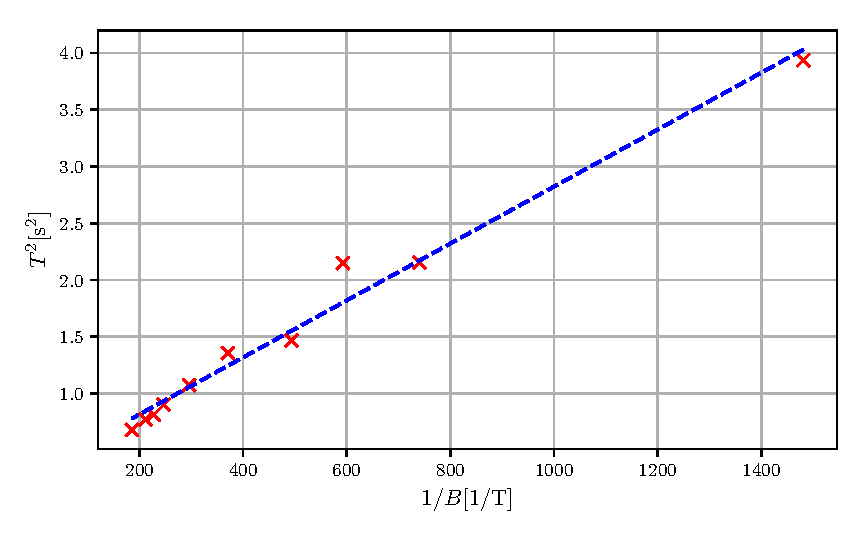
\includegraphics{schwing.pdf}
  \caption{Temperaturen der Wärmereservoirs aufgetragen gegen die Zeit.}
  \label{fig:schwing}
\end{figure}
Daraus folgt eine Steigung von $m=0.00251/pm 0.00012$ für die lineare Ausgleichsgerade.
Das magnetische Moment lässt sich dann nach Formel berechnen:
\begin{equation}
  \mu_{Dipol}= \frac{\pi^2 \cdot J_{Kugel}}{m}=(0.59)\si{\ampere\meter\squared}
\end{equation}
\subsection{Bestimmung des magnetischen Moments über Präzession}

\section{Diskussion}
\label{sec:Diskussion}
Aus den hier erhaltenen Werten lässt sich folgern, dass die Messung unter Ausnutzung der Gravitation und die Messung über die Präzession am geeignetsten sind.
Ihre Ungenauigkeiten befinden sich in der gleichen Größenordnung, sowie auch der Wert des Dipolmoments.
Bei der Messung über die Präzession sind jedoch viele systematische Fehlerquellen enthalten.
Deshalb ist die Aussagekraft des so bestimmten Werts fragwürdig.
Die Abweichung des durch Schwingungsdauer gemessenen Werts lässt sich einerseits, durch die mögliche Varianz der Auslenkungen erklären, andererseits kann es auch sein, dass die Kugel nicht vollständig in nur einer Ebene geschwungen ist.
Somit folgt , dass die Messung unter Ausnutzung der Gravitation am geeignetsten ist, da sie die geringsten systeamtischen Fehler aufweist.


\printbibliography{}

\end{document}
